\section{Methods}
\subsection{Data Collection}
our study depends on three types of data: (1) Large repositories that include C++ source code which could contain buffer overflow vulnerabilities, (2) Static analysis tools that could analyze the source code, and (3) Vulnerability reports that are generated from running static analysis tools against the source code of the repositories. In the following section, a detailed description about each conducted step.
\newline
\subsubsection{\textbf{Selecting Projects}}
Our goal was to study the effectiveness of static analysis tools through studying the historical data of large repositories. Therefore, GitHub was chosen to conduct such an analysis. We used RepoReapers dataset \cite{Reporeapers2016} to retrieve our dataset. As we wanted to focus on C++ projects, we filtered RepoReapers dataset to include only projects that are written in C++. Since our analysis depends on the historical data in these large repertoires, we needed to mine projects that have adequately long historical data. Thus, we selected projects in RepoReapers dataset that have the most stars, which indicates the projects popularity. As those projects are more likely to be more active and thus have more number of commits. Then, we ordered RepoReapers dataset by the highest number of stars, then we selected the top 10,000. After that, we randomly selected 400 projects from the 10,000 list. When we mined the chosen repositories from GitHub, we applied some criteria to ensure the robustness of our dataset. For instance, we built a tool to ensure that retrieved projects are indeed C++ projects. We found that 27 of mined projects are not C++ projects and thus we removed them from our dataset; and selected new ones randomly from the 10,000 list. In addition, we excluded projects with fewer than 40 commits, we found that 17 projects have less than 40 commits which were excluded then. Also, all mined projects were tested to see whether they adopt cmake build system, as we planed to expand our analysis to test more advanced static analysis tools that analyze projects based on that build system. We found 270 projects are not adopting cmake build, thus we continently cloned projects from the 10,000 list to construct our dataset. In all cases that we needed to clone new project from the 10,000 list, we ensured that new selected new one that are not included in our 400 list. For this study, we run our analysis against only 40 projects that were chosen randomly.
\newline

\subsubsection{\textbf{Gathering Static Analysis Tools}}
We gathered three open source static analysis tools that discover buffer overflow. Our study tests the following tools that support C++:  Cppcheck \cite{Torri2010}, Flawfinder \cite{Torri2010}, and RATS \cite{Torri2010}.  Table \ref{C++SAT} summarizes all tested tools and their versions. 


\begin{table}[ht]
\centering
\scriptsize
\caption{The Studied free and open source static analysis tools that detect buffer overflow in C++}
\label{C++SAT}
\begin{tabular}{||p{1.5cm}|p{1cm} p{2.6cm}p{1.2cm}||}
\hline
 \textbf{Tool Name} &  \textbf{Language} &\textbf{Inference Algorithm} &  \textbf{Version Number}\\

\hline\hline

RATS & C/C++ &String pattern matching &  2.4\\  
Flawfinder & C/C++ &String pattern matching &  1.31 \\  
Cppcheck  &C/C++ & Constraint-based & 1.72 \\ \hline

\end{tabular}
\end{table}


\subsubsection{\textbf{Collecting Vulnerability Information}}
After gathering some large repositories and static analysis tools, we needed to run static analysis tools against those repositories. We wanted to get all possible warnings regarding buffer overflow and calculate some metrics regarding the statics analysis tools. The main research question is to study the effectiveness of static analysis tools which has been studied previously. However, our approach is different than traditional research papers that studied the same topic. While they conducted the analysis on test cases with having true positive warnings in advance, which makes it easy to measure precision, recall, etc., we do not.
The main idea of our work is to study the historical records of the repositories to extract true and false positives vulnerability warnings. We can do so by running static analysis tools against different versions of a repository. Hence, we need to trace how and when a vulnerability was introduced and removed through time; and based on this kind of information we can decide whether a given vulnerability is false positive or true positive. Analyzing a repository at different points of time would insure that our analysis not only could trace a bug report at different times but also to catch any vulnerability that is introduced at any time.

We first intended to run the static analysis tools against all commits of a repository. However, we found that this will be impractical because this would consume more resources and time when analyzing very large repertoires, which sometimes include commits up to hundreds of thousands. Then, we thought about running static analysis tools against different releases (e.g., using git tag) which could be more practical. However, we found that this solution could not be generalized to all repositories. This is because that not all projects use this functionality to annotate release points. In fact, we found that most often the studied repositories do not use this functionality at all( as Table \ref{stat} shows that the mode of the n\_release which indicates the number of tagged release in the studied repositories is 0). 

Therefore, we had to come up with a solution that analyze a repository at different points of time and at the same time should not need to use heavy resources.  Thus, we have decided to run static analysis tools on each repository at six-monthly intervals starting from the initial date of each project and ending with last updated date of a project when we cloned the dataset.  We called each tested commit a \textbf{checkpoint}, so each repository has \textbf{n} checkpoints based on its age ( Table \ref{stat} shows statistic about  projects ages  and the number of checkpoints).


In the following section, a detailed description about steps that were conducted to generate vulnerability hit lists as illustrated in Figure~\ref{cyc}. 

\begin{figure} [h!]
\centering
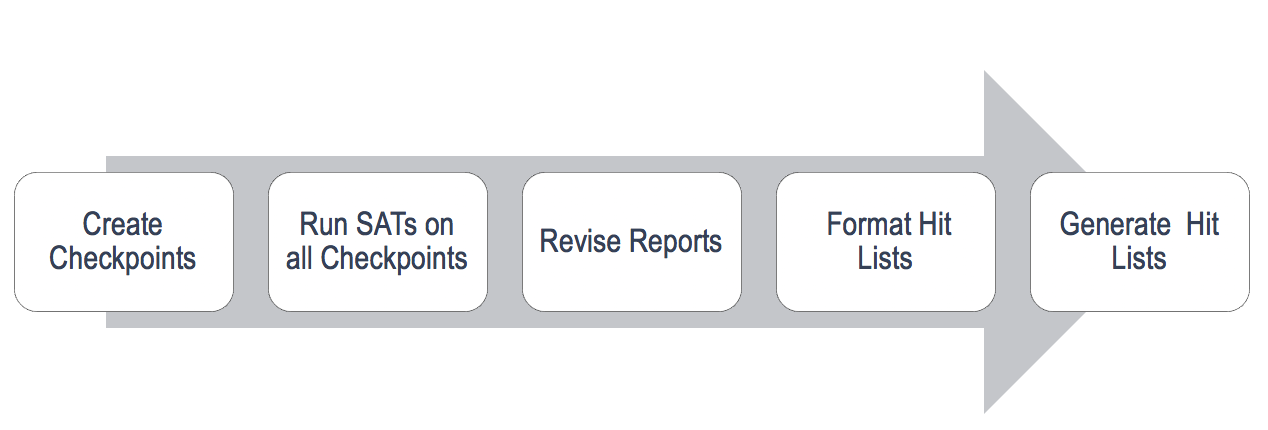
\includegraphics[height=1in, width=3in]{hit.png}
\caption{Steps that were conducted to generate hits lists reports}
\label{cyc}
\end{figure}

\begin{itemize}[leftmargin=*]
\item \textbf{ Step 1: Create Checkpoints}
The first task that we achieved is to create a list of candidate checkpoints for each repository. We fist dumped a list of commits dates for each repository. Then, we started from the date of the last commit and calculated the date differences of previous commits until we reached a commit with six month interval. Once we identify a commit with six months interval, we store both the commit hash (SHA value) and date. From the last stored commits that have six months interval we continue doing the same thing as we calculate the date difference with the remaining dates in the list until we reach the last date. By completing this step, we generating a list of \textbf{n} checkpoints for each repository depending on the age of that repository. Table \ref{stat} shows some statistics related to the project age (proj\_age) and number of checkpoints (n\_checkpnt) in our dataset.

\item \textbf{ Step 2: Run SATs on all Checkpoints}
Now each repository has a list of checkpoints. Hence in this step, we  run all static analysis tools (SATs) on all checkpoints of each tested repository.  So, when the analysis is run in a repository,  we first convert the working tree and the source code to match a given checkpoint (by performing subsequent \textbf{ git checkout commit-sha-value} on all considered checkpoint).  With each checkpoint we collected a number of metrics about that checkpoint, such as  number of source files (n\_src\_files), number of header files (n\_h\_files ), and line of codes (LOC) (See Table \ref{stat} for more information. We only considered the source and header files that are written in C++. So, we filtered the source files to only include files that have an extension of (C, cpp, CPP, cxx, cc, CC, cp, c++)  and header files that have an extension of(h, hh, hpp, H). This filtration also help us to direct static analysis tools to only analyze C++ files, as some of them (e.g., RATS) do multiple languages analysis. Indeed, our dataset includes projects that  include multiple programming languages, thus we wanted to restrict the analysis on C++ files only.

\item  \textbf{ Step 3: Revise Reports}
We revised all reports in terms of vulnerability type and tested file type. Regarding vulnerability type, each static analysis tool could detect different types of bugs. However, we only interested in buffer overflow vulnerabilities. Therefore, we had to provide a solution to only consider buffer overflow vulnerabilities. We goaled to do so with the initial analysis to reduce the required resources and the running time. Each tool was designed differently and generate the vulnerabilities in a variant way. Hence, we had to understand how these tools are generating their hit list in the first place.  Since, all studied tools are open source, that task was achievable. We found that Flawfinder includes 169 number of rules (primarily dangerous function names) in C/C++. Flawfinder allow users to specify which types of vulnerability to be analyzed. It is not obvious though, as Flawfinder does not declare that clearly.  However, by digging deeply into the source code, the documentation, and other files in Flawfinder package, we found a way of doing so. Flawfiner reports vulnerabilities based on the CWE/SANS top 25 list. It uses CWE identifiers to report any bug that matches the CWE pattern. For example, CWE-120 represents the classic buffer overflow vulnerability, which is copying the buffer without checking the size of the input. Thus, we used \textbf{--regex} flag to retrieve only CWE that are related to buffer overflow vulnerabilities. The CWE that we included are the following:


\begin{enumerate}
\item CWE-120: Classic buffer overflow 
\item CWE-126: Buffer Over-read
\item CWE-20: Improper Input Validation
\item CWE-119: Improper Restriction of Operations within the Bounds of a Memory Buffer
\item CWE-785: Use of Path Manipulation Function without Maximum-sized Buffer
\item CWE-676: Use of Potentially Dangerous Function
\end{enumerate} 

Other flags that used with Flawfinder are: \textbf{--quiet} to suppress all irrelevant information that are provided by the tool, such as which files are being analyzed while the tool is running. Also, we used \textbf{--context} flag to show which line of code that includes the vulnerability. This peace of information is very critical in our analysis, as most of the analyses depend primarily on it. In addition, we used \textbf{--dataonly} to obtain only the results and discard other information such as the headers and footers of the analysis. Finally, we used \textbf{--singleline} to show each bug report in single line, this would help us to create more neat hit list report.


With RATS, there is no way to specify which type of vulnerability to be analyzed. In fact, RATS uses different vulnerability database for each programming language. However, the tool provide a way to specify an alternate vulnerability database. So, we created our own vulnerability database that include buffer overflow vulnerabilities. In particular, we copied the original database and removed all other types of vulnerabilities other than buffer overflow vulnerabilities. We found that Rats includes 310 vulnerabilities reports, and only 213 for buffer errors.

When we run RATS, we use the flowing flags:  \textbf{-x} to avoid loading the default databases. Also, we used \textbf{-d} to load our alternate vulnerability database. 
In addition, we utilized  \textbf{--quiet} to suppress other ongoing irrelevant output, \textbf{ --resultsonly} to discard header, footer, and status information that are generated by default., and \textbf{---context} to show which line of code that include the vulnerability.

Cppcheck also could help to chose which bug report to be produced. The way that Cppchek does this is by allowing to suppress unwanted bug reports. It provide \textbf{--suppressions-list} flag and a user can generate a file that include unwanted bug warnings. We could get a list of all possible warnings in Cppcheck by running \textbf{--errorlist}. We found that Cppchek has 231 errors and only 31 are related to buffer overflow. So we created a list with 200 bug that should be suppressed.



We use a number of other Cppcheck flags as  well. We used \textbf{--quiet} to suppress all progress reports. Also, we used \textbf{ --language} flag to direct Cppcheck to check all files in the given language which is C++ in our case. In addition, \textbf{--template} was used to format the output report of the tool to be consistent with our report format. The following section include more information about our report format.  


Regarding the tested file type, we only interested in source code file that represents the program code and not source code files for test purposes. Therefore, in this step we removed all warnings that indicate that a given vulnerability happened in source code for test purposes. We inferred that from the file path which usually include any form of ``test'' keyword in it.
 
%"cppcheck:{file}:{line}:{severity}:{id}:{message}" 


\item \textbf{ Step 4: Format Hit Lists}
Each static analysis tool has its own format when it generates its hits list. When we analyzed a repository, we wanted to store all warnings of bugs at each checkpoint in one file.  Therefore, all warnings by all studied static analysis tools should be saved in one file to process them later. However, because our analysis depends mainly on processing these hit lists, we wanted to produce consistent and united format. This will make our analysis more easer and precise. Therefore, we generated our own formatted hits list as follow:
\newline

\fbox{\begin{minipage}{24em}
Tool Name : File Path : Line Number :Severity: Vulnerability Type : Context 
\end{minipage}}\\

By producing this kind of report, we insure that each bug warning has a its own signature.  \textbf{Tool Name} helps us to keep track which tool that produces such warning. This will help us to measure the precision and false positive rate for each tool.  \textbf{File Path} allow us to analysis and track the same file in different checkpoints in order to decide whether a given warning is false or true positive.  
\textbf{Line Number}  aids  us to insure that a given warning  is the same warning that appears in the same file but in other checkpoints. Also, sometime we could encounter situation where exact vulnerability that happen in the same file twice with different line numbers. Thus, line number would help us to differentiate between different vulnerabilities that hold the same context.  \textbf{Severity} this part of the report is generated by the studied static analysis tools by default. We thought that it could be beneficial to keep track of how the tool is evaluating a such  warning. Also, it could gives us more information when we extract the pattern of true positive warnings. Similarly \textbf{Vulnerability Type} also would aid us  to extract the pattern and the frequency of such vulnerability in real world. Finally  
\textbf{Context} is a very important element of the report. It could not only  help us to identify the uniqueness of the bug, but also it could serve  to reveal more information about the bug pattern, such as does it contains pointer operations?, what is the container of the bug?, what is the memory location?, etc.
 
 \item \textbf{ Step 5: Generate Hit Lists}
The last step was to generate hit lists of all static analysis tools against all studied repositories. All generated reports follow the format that was mentioned in Step 4.  Each repository includes \textbf{n} reports for each checkpoint.  We tested 40 repositories that include 341 checkpoints in total which means that we run all three static analysis tool 341 times. Also, in this step we collected some metrics about the warnings that were generated by each static analysis tool and the running times.
\begin{table}[ht]
\centering
\scriptsize
\caption{Summary statistics on the various metrics related to the studied static analysis tools.}
\label{SAT}
\begin{tabular}{||p{1.4cm}|p{.8cm} p{.7cm} p{.2cm} p{.7cm} p{.2cm} p{.5cm} p{.9cm}||}
\hline
\textbf{Statistic} & \textbf{Sum} & \textbf{Max} &	 \textbf{Min} 	& \textbf{Mean} 	&	 \textbf{Mode} 	& \textbf{Median} 	&  \textbf{Sst.Dev}\\
\hline\hline
RATS\_BO  & 47315 & 2582 &	0&	163.15	&0	&7&	406.73 \\
Flawfinder\_BO &96733 &3886 &	0 &	333.56 &	1	&16	&682.84 \\
Cppcheck\_BO &0 & 0	&0&	0	&0	&0	&0 \\

RATS\_rt & 264083 &12474&	15	&910.63&	104&	288.5	&1966.96\\

Falwfinder\_rt & 702497 &20014	&76&	2422.40&	588	&972.5&	4154.88 \\
Cppcheck\_rt &16551768 &2259102&	50	&57075.06&	58&	2089&	159674.17\\

\hline


\end{tabular}
\end{table}

Table \ref{SAT} shows some metrics regarding the detected vulnerabilities. These vulnerabilities are not unique meaning that one vulnerability could appear in different checkpoints, thus this table show the sum of all reported vulnerabilities. 
RATS\_rt , Falwfinder\_rt, and Cppcheck\_rt indicate the running time of each tool.  The running time in this table is measured in milliseconds. 





\end{itemize} 



%Then we build a tool that analyze these project by running open source static analysis tools that are shown in Table I. So, in general we will mainly use use source codes, commits, meta-data



\subsubsection{\textbf{Collecting Metrics Information}}
While we examined the studied repositories, we measured multiple metrics regarding the repositories to get better a better insight about our dataset. Table \ref{stat} shows some statistics related to the project age in months (proj\_age), number of commits (n\_commits),  number of checkpoints (n\_checkpnt),number of release (n\_release), number of the source files (n\_src\_files), number of header files (n\_h\_files), and line of code (LOC) of all studies repositories in our dataset. All statistics were collected using datamash tool \cite{datamash}.


\begin{table}[ht]
\centering
\scriptsize
\caption{Summary statistics on the various metrics related to the studied repositories.}
\label{stat}
\begin{tabular}{||p{1cm}|p{.5cm} p{.3cm} p{1cm} p{.6cm} p{.8cm} p{1cm}||}
\hline
\textbf{Statistic} & \textbf{Max} &	 \textbf{Min} 	& \textbf{Mean} 	&	 \textbf{Mode} 	& \textbf{Median} 	&  \textbf{Sst.Dev}\\
\hline\hline
proj\_age & 155 &	12	& 46.95	 & 12	& 35.5	& 31.1 \\                n\_commits & 8530	& 40& 	922.4	& 1651	& 392.5	& 1621.5 \\ 
n\_checkpnt & 42& 2	&8.5	&5&	6	&7.04  \\
n\_release &31	&0&	6.2	&0	&2.5 &	9.05  \\
n\_src\_files &899	&1	& 90.7 &	1 &38.5	&149.2 \\
n\_h\_files & 1017&	0&	122.4	&0	&52	& 212.7\\
LOC & 808325	& 5	&72831.3 &	90595	&23049.5&	143163.3  \\
\hline


\end{tabular}
\end{table}


